% !TEX encoding = UTF-8
% !TEX TS-program = pdflatex
% !TEX root = ../Tesi.tex
% !TEX spellcheck = it-IT

%************************************************
\chapter{Hybrid Reciprocal Velocity Obstacle}
\label{cap:hrvo}
%************************************************

Con le nozioni esplicitate precedentemente per VO e RVO, HRVO permette di diminuire le oscillazioni e creare traiettorie \textit{smooth}, (osservare l'immagine del capitolo per comprendere alcuni aspetti sulla CL di RVO).

\section{Hybrid Reciprocal Velocity Obstacle}

Per l'agente {\bfseries\textit{A}} e {\bfseries\textit{B}}, se {\bfseries\textit{v}\ped {A}}  \'e sulla destra del \textit{centreline} (CL) di \textit{RVO}\ped{A,B}, il quale per simmetria {\bfseries\textit{v}\ped {B}} sar\'a sul lato destro della \textit{centreline} di \textit{RVO}\ped{B,A}, noi speriamo che \textit{A} scelga la velocit\'a sulla destra di \textit{RVO}\ped{A,B}. Per favorire questo, l' \textit{RVO} \'e allargato sostituendo il bordo sul lato dove desideriamo che il robot non passi, in questo caso il lato sinistro, dal bordo della \textit{VO}\ped{A,B}. L'apice della risultante del cono corrisponde al punto di intersezione tra il lato destro della \textit{RVO}\ped{A,B} e il lato sinistro della \textit{VO}\ped{A,B}. Se la {\bfseries\textit{v}\ped {A}} st\'a a sinistra della \textit{centreline} (CL), noi replichiamo la stessa procedura scambiando la sinistra con la destra. Per questo \'e chiamato ibrido tra RVO e VO, \textit{HRVO}\ped{A,B}.  

\subsection{New Velocity}
La computazione della nuova velocit\'a chiamata {\bfseries\textit{v}\ap{new}\ped{Ai}}, al di fuori della combinazione dei HRVO, \'e la minima distanza tra la velocit\'a corrente e la velocit\'a preferita:

\begin{gather}
v^{new}_{Ai}= argmin_ {v \notin HRVO_{Ai}} norm(v - v^{pref}_{Ai}).
\end{gather}

Per computare tale velocit\'a viene utilizzato un algoritmo chiamato ClearPath, combinando tutti gli \textit{HRVO} come intersezioni di segmenti, dove le coppie dei punti di intersezione all'interno del \textit{HRVO} vengono scartati. Le possibili velocit\'a ammissibili saranno tutte le intersezioni dei coni sul bordo di \textit{HRVO}. Aggiungendo la proiezione della velocit\'a preferita, la nuova velocit\'a sar\'a selezionata tra la minima distanza che c'\'e tra le velocit\'a ammissibili (intersezioni dei coni) e la velocit\'a preferita del robot {\bfseries\textit{v}\ap{pref}\ped{Ai}} . 
\\ Se non si riesce a trovare una possibile velocit\'a ammissibile, la procedura viene ripetuta riutilizzando l'algoritmo del ClearPath.

\begin{figure}
\centering 
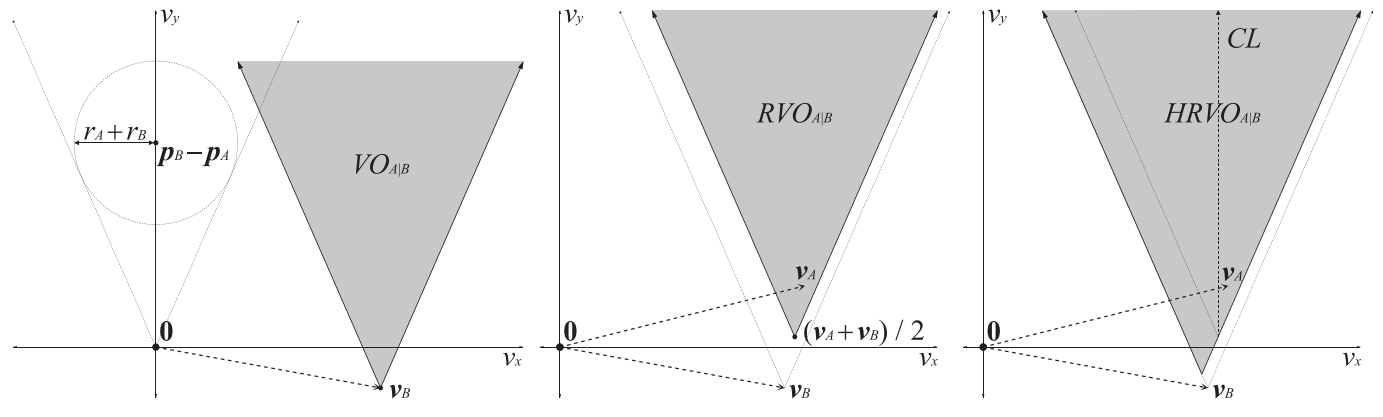
\includegraphics[width=0.8\columnwidth]{hrvo2} 
\caption[Costruzione del HRVO rispetto gli algoritmi precedentemente descritti]{Costruzione del HRVO rispetto gli algoritmi precedentemente descritti}
\label{fig:hrvo} 
\end{figure}

\subsection{Descrizione dell'algoritmo}

Descrizione dell'implementazione dell'algoritmo HRVO:
\\
\\
\begin{lstlisting}
Input A = List of robots, O = List of obstacles
loop
for all Ai in A do
Sense pAi and vAi
for all Aj E A such that j != i do
Sense pAj and vAj
Construct VOAi|Aj and RVOAi|Aj
Locate centerline CL of RVOAi|Aj
if vA is right of CL then
Replace left side of RVOAi|Aj with left side of VOAi|Aj to construct HRVOAi|Aj
else
Replace right side of RVOAi|Aj with right side of VOAi|Aj to construct HRVOAi|Aj
end if
Expand HRVOAi|Aj to HRVOAi|Aj
end for
for all Oj E O do
Sense pOj and vOj as appropriate
Construct VOAi|Oj
Expand VOAi|Oj to VOAi|Oj
end for
Construct HRVOAi from all HRVOAi|Aj and VOAi|Oj
Compute preferred velocity vprefAi
Compute new velocity vnewAi !E HRVOAi closest to vprefAi
Compute control inputs from vnewAi
Apply control inputs to actuators of Ai
end for
end loop

\end{lstlisting}











